\capitulo{6}{Aspectos relevantes del desarrollo del proyecto}

Este punto es el más importante de la memoria, ya que contiene, de manera descriptiva y detallada, el proceso seguido desde el inicio hasta el fin del proyecto. Para una mejor comprensión, el orden de los subpuntos que contiene este apartado están ordenados de manera cronológica. Además, se hablará acerca de los problemas surgidos, soluciones tomadas y alguna posible alterativa. 

Antes de entrar en materia, cabe destacar que la primera idea que teníamos por parte de la empresa, es que querían comprobar, si con los niveles mínimos y máximos de zinc, la decisión por parte del operario era la correcta acerca de si la bobina era válida o no. Y tras comprobar los niveles y clasificar de nuevo las bobinas, crear una red neuronal capaz de clasificar futuras bobinas.

Pero más adelante se nos comentó que las decisiones por parte del operario sobre si la bobina era válida o no, eran las correctas, y su interés estaba en obtener un modelo que con los valores capturados por los sensores se pueda predecir, sin necesidad del operario, si la bobina es correcta o no.

\section{Carga de Datos y Evaluación de Bobinas}
En esta primera fase, lo primero que se hizo fue cargar los datos que nos había cedido la empresa, y que se encontraban en una base de datos de MySQL, para realizar una sencilla exploración de datos y saber con exactitud el número de datos con el que se contaba.

Antes de nada, comentar que la empresa nos cedió datos de bobinas medidas por sensores 1D y 2D, por lo que se cuenta con dos tipos de datos. Además, de los sensores 1D se contaba con dos parejas de sensores diferentes (cada pareja tenía un sensor que media la capa de arriba y otro la capa de abajo de la bobina.) De manera gráfica se entiende muy fácilmente cómo son los datos con los que se cuenta. En la Figura \ref{f:datos1D}se puede ver como son los datos 1D, que no dejarían de ser más que un \emph{array} de una dimensión. Con respecto a los datos 2D, Figura \ref{f:datos2D}, se pueden interpretar como una matriz de 9 filas y el número de columnas cambiantes según cada bobina. Además, a cada celda, tanto en datos 1D como 2D, se le conoce como teja.

\begin{figure}[h]
 \centering
  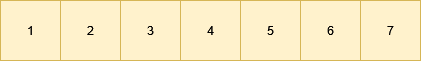
\includegraphics[width=0.9\textwidth]{img/1D.png}
 \caption{Ejemplo estructura datos 1D}
 \label{f:datos1D}
\end{figure}

\begin{figure}[h]
 \centering
  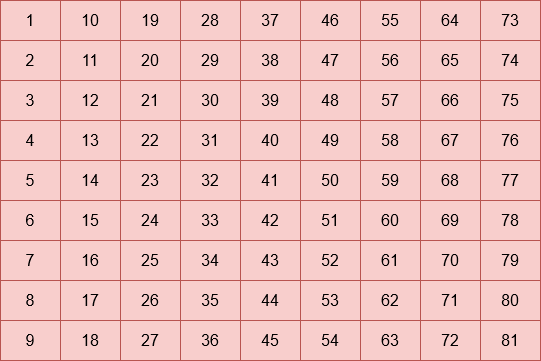
\includegraphics[width=0.9\textwidth]{img/2D.png}
 \caption{Ejemplo estructura datos 2D}
 \label{f:datos2D}
\end{figure}




Una vez explicada la estructura de los diferentes datos, añadir que se cuentan 1160 bobinas previamente evaluadas por un operario, con 115972 registros de los datos 1D, correspondientes a las diferentes tejas medidas, y con 127312 registros de los datos 2D.

Ahora que ya se comprendían los datos, era turno de evaluar cada bobina. Para ello se creó una función que evaluaba cada bobina con sus diferentes tejas y se comprobaba que en cada una de ellas se cumplían con los requisitos mínimos y máximos de zinc correspondientes a la bobina. Toda esta evaluación se realizaba para cada uno de los sensores, y además, se contaban el número de fallos, es decir, el número de tejas que no cumplía los requisitos, y si se había producido algún calibrado. Esto último consiste en reiniciar los sensores y sus mediciones serían 0 en ese registro, pero que no indica que la teja este mal. 

En la Figura \ref{f:evalua1} se muestra el resultado obtenido para las dos primeras bobinas, en las que se indica la ID de la bobina (\emph{COILID}), la ID del sensor (\emph{MID}), la clase del operario y la clase obtenida por el proyecto, y finalmente el número de fallos y el número de calibrados, si es que se ha producido alguno.

\begin{figure}[h]
 \centering
  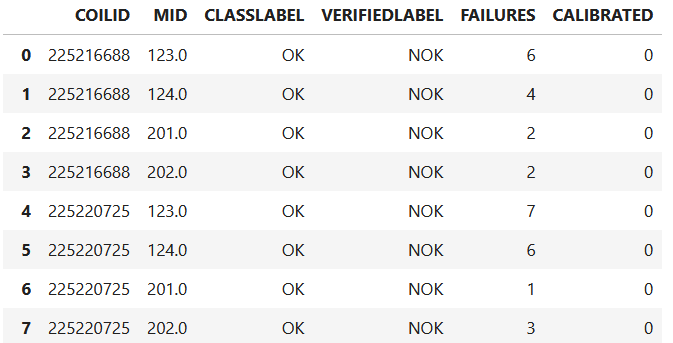
\includegraphics[width=0.9\textwidth]{img/evalua1.PNG}
 \caption{Ejemplo de Evaluación de 2 Bobinas}
 \label{f:evalua1}
\end{figure}

Finalmente, en esta fase se mostraron las estadísticas de las clases obtenidas por los operarios y por el proyecto. A continuación, se puede ver en detalle:
\begin{verbatim} 
        Los valores de los operarios han sido:
         OK    3340
        NOK    1300
        
        Los valores que se han obtenido son:
         OK      98
        NOK    4542
\end{verbatim}
A simple vista se puede observar que había una anomalía, y como ya se había comentado previamente, se debía a esa pequeña confusión que hubo en un primer lugar con la empresa, y que tras una nueva reunión, se dijo que estas bobinas sí que estaban ya bien clasificadas previamente por un operario y que simplemente era necesario proceder a la construcción de una red neuronal. 

También se puede ver como el conjunto de datos está desbalanceado (mirando las estadísticas de las clases de los operarios), ya que la clase OK es la mayoritaria, con aproximadamente un 72\% de los datos, mientras que la clase NOK es la minoritaria con aproximadamente el 28\% de los datos.

\section{Visualización de las Bobinas}
En esta segunda fase, se realizó la parte correspondiente a representar gráficamente los datos 1D junto con los valores en los que tiene que encontrarse el zinc. Para ello, se realizó un desplegable con las IDs de las diferentes bobinas, y que al seleccionar una, se mostraran los gráficos de los cuatro sensores. 

La Figura \ref{f:visu} muestra un ejemplo de visualización de las cuatro gráficas, correspondientes a los diferentes sensores, junto con los diferentes valores de zinc medidos; además de una línea roja que representa el máximo o el mínimo de zinc en cada caso.

\begin{figure}[h]
 \centering
  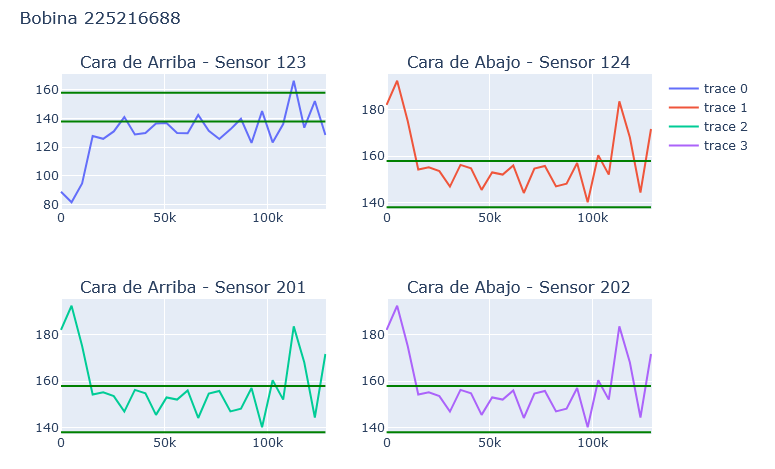
\includegraphics[width=0.9\textwidth]{img/visuaBobi.PNG}
 \caption{Ejemplo de Visualización para una Bobina}
 \label{f:visu}
\end{figure}

\section{Obtención de las Características de las Bobinas}
Esta tercera fase se ha centrado en la obtención de las principales \emph{features} de cada bobina, junto con la codificación del mapa que forman los datos 1D o 2D, para posteriormente ser utilizados en la red neuronal. 

En primer lugar, las características o \emph{features} que se han obtenido para cada bobina han sido las siguientes:
\begin{itemize}
    \item \textbf{ZNMAX\_FAILURES:} se corresponde al número de tejas que tiene una capa de zinc superior al estipulado. Los fallos se contarán desde que hay un fallo hasta que se encuentra una teja correcta, no un fallo por cada teja con un defecto.
    \item \textbf{ZNMIN\_FAILURES:} es el número de tejas de la bobina que tiene menos zinc del mínimo estipulado. Los fallos también se cuentan con el mismo criterio que el caso anterior.
    \item \textbf{CALIBRATED:} se corresponde al número de tejas en las que se ha producido un calibrado (reinico de los sensores).
    \item \textbf{TOTAL\_TILEID:} indica el número total de las tejas que tiene la bobina.
    \item \textbf{L\_DIS:} contiene el número de tejas que hay desde el inicio de la bobina hasta el último fallo antes de la mitad de la bobina.
    \item \textbf{R\_DIS:} indica el número de tejas que hay desde el fallo más cercano a la mitad y el final.
\end{itemize}

En segundo lugar, la codificación del mapa de las bobinas se ha llevado de la siguiente manera:
\begin{itemize}
    \item \textbf{1:} en caso de que la teja tenga más zinc del máximo.
    \item \textbf{0:} indica que el valor de zinc de la teja está dentro de los mínimos y máximos.
    \item \textbf{-1:} correspondiente a una teja que tenga menos zinc del mínimo necesario.
\end{itemize}

Cabe destacar que, tanto las \emph{features} como la codificación del mapa de la bobina son iguales tanto para los datos 1D como 2D. Para visualizarlo mejor, la Figura \ref{f:fea1d}, muestra un ejemplo de salida de datos 1D. En ella se pueden ver todos los atributos anteriormente mencionados para una misma bobina y los valores obtenidos por parte de los 4 sensores diferentes.

\begin{figure}[h]
 \centering
  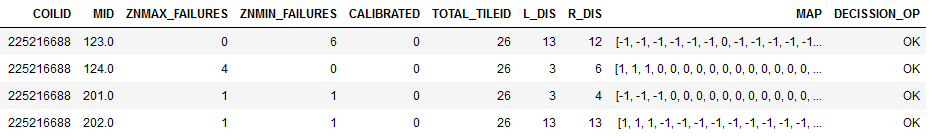
\includegraphics[width=1\textwidth]{img/fea1D.PNG}
 \caption{Ejemplo de características obtenidas para datos 1D}
 \label{f:fea1d}
\end{figure}

Por otro lado, tenemos la Figura \ref{f:fea2d}, que muestra, para la misma bobina que en la Figura anterior, las características obtenidas para los sensores 2D. En dicha figura, se puede ver como el mapa es también un \emph{array}, ya que por comodidad se ha guardado así, pero posteriormente, cuando se lea, se reconstruirá en forma de matriz.

\begin{figure}[h]
 \centering
  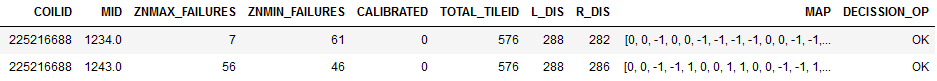
\includegraphics[width=1\textwidth]{img/fea2D.PNG}
 \caption{Ejemplo de características obtenidas para datos 2D}
 \label{f:fea2d}
\end{figure}

Finalmente, en esta tercera fase, se han guardado las características obtenidas de los datos 1D y 2D en una base de datos. Para ello se han creado dos tablas, FEATURES\_1D y FEATURES\_2D, donde se almacena todo el contenido previamente calculado.

\section{Pruebas CNNs}
Una vez se contaba con los datos preparados, en este cuarta fase se realizaron diferentes pruebas en la construcción de CNNs de la librería \emph{TensorFlow}, con el fin de poder familiarizarse con su uso. Además, y antes de empezar a construir redes neuronales, había que preprocesar los datos para poder usarlos. También, indicar que en esta fase las pruebas fueron únicamente con datos 1D.

En primer lugar, se cargaron los mapas codificados de las bobinas 1D, obtenidos en la tercera fase, y se decidió unir en un único \emph{array} cada par de sensores, es decir, unir los mapas de los sensores 123 y 124 y, por otro lado, los sensores 201 y 202, con el fin de poder utilizar las convoluciones 1D sobre los datos.

A continuación, sobre estos nuevos mapas unidos, se aplicó la técnica de \emph{padding}, que se basa en rellenar los datos con un valor para que todos ellos tengan las mismas dimensiones, ya que es necesario para las redes neuronales que se van a construir. En este caso, se rellenaron los datos con 0, hasta que todos los datos tuvieran una longitud de 208, puesto que fue el valor más grande encontrado dentro del conjunto de datos.

Ahora ye se contaba con los mapas preparados para ser usados, pero antes había que transformar la clase de \emph{string} a \emph{int}. Dicha transforamción fue: un 0 para la clase OK y un 1 para la clase NOK.

En este punto ya se cuenta con los datos listos, por lo que era turno de construir modelos. En primer lugar, se crearon modelos individuales para aprender como funciona su construcción, la Figura \ref{f:modelo1}, muestra un ejemplo de construcción. Aunque, como suele ser habitual en estos casos para generar modelos, se utilizará la estrategia de validación cruzada  o \emph{cross validation} para poder evaluar los diferentes modelos construidos de manera más precisa y robusta.

\begin{figure}[h]
 \centering
  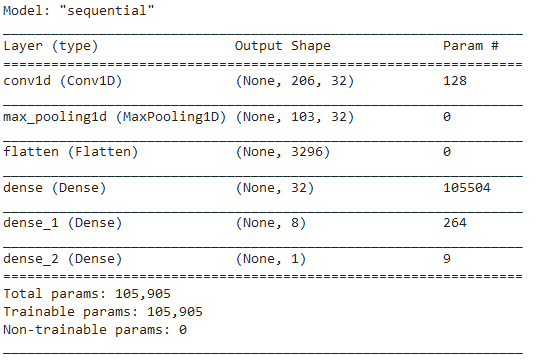
\includegraphics[width=0.8\textwidth]{img/modelo1.PNG}
 \caption{Ejemplo de Construcción de Modelo}
 \label{f:modelo1}
\end{figure}

Finalmente, en esta fase de pruebas también se decide hacer pruebas utilizando alguna técnica para ajustar el conjunto de datos desbalanceado. En este caso se opta, debido al bajo número de registros, a realizar un sobremuestreo de los datos, y más concretamente aplicar la técnica SMOTE.

SMOTE (\emph{Synthetic Minority Oversampling Technique}) se basa en crear más ejemplos de la clase minoritaria de manera sintética. Para ello, busca dos ejemplos que estén próximos y genera uno nuevo con datos intermedios entre los dos ejemplos. Este proceso se repite varias veces hasta que el conjunto de datos se encuentra equilibrado.

Para concluir esta fase, indicar que los mejores resultados se consiguieron con datos a los que se les había aplicado el sobremuestreo, por lo que se decidirá usar este conjunto de datos en la siguiente fase.

\section{Generación, Obtención y Evaluación CNNs}
En esta quinta y penúltima fase, es turno de realizar un conjunto de experimentos, ahora que ya se sabe como crear modelos, para ver cuál es el que consigue mejores resultados para usarse en la aplicación del proyecto.

En primer lugar, se reconstruirá el mapa de los datos 2D, puesto que el de los datos 1D es el mismo que el comentado en la anterior fase. Para ello, se carga el \emph{array} que contenía todos los datos y se pasa a una matriz de 9 filas y de nuevo se aplica la técnica de \emph{padding}, para que todos los datos tengan el mismo número de columnas, rellenando con ceros.

Además, también se utilizarán las \emph{features} generadas en la tercera fase con el fin de ver si pasándole al modelo el mapa y sus características normalizadas se obtienen mejores resultados. También, se probará si para estos datos funciona mejor un \emph{Random Forest} que se construirá para cada experimento con los atributos normalizados y las predicciones de los modelos.

En segundo lugar, se ha buscado el criterio de clasificación, ya que en un primer lugar se puede pensar qué 0.5 sería el valor correcto para diferenciar ambas clases, pero la realidad es que en cada problema el criterio puede ser totalmente distinto. Para ello, se ha aplicado la técnica de validación cruzada y se ha construido un modelo y se han probado 6 criterios diferentes de clasificación: 0.2, 0.3, 0.4, 0.5, 0.6, 0.7. 

Para cada uno de los criterios probados se ha construido su curva ROC y se ha calculado su AUC para ver cuál de todos ellos es el mejor. Tras realizar varias pruebas, se ha llegado a la conclusión que el mejor parámetro es 0.3, tal y como se puede ver en la Figura \ref{f:curvasROC}, donde este criterio es el que tiene mayor AUC.

\begin{figure}[h]
 \centering
  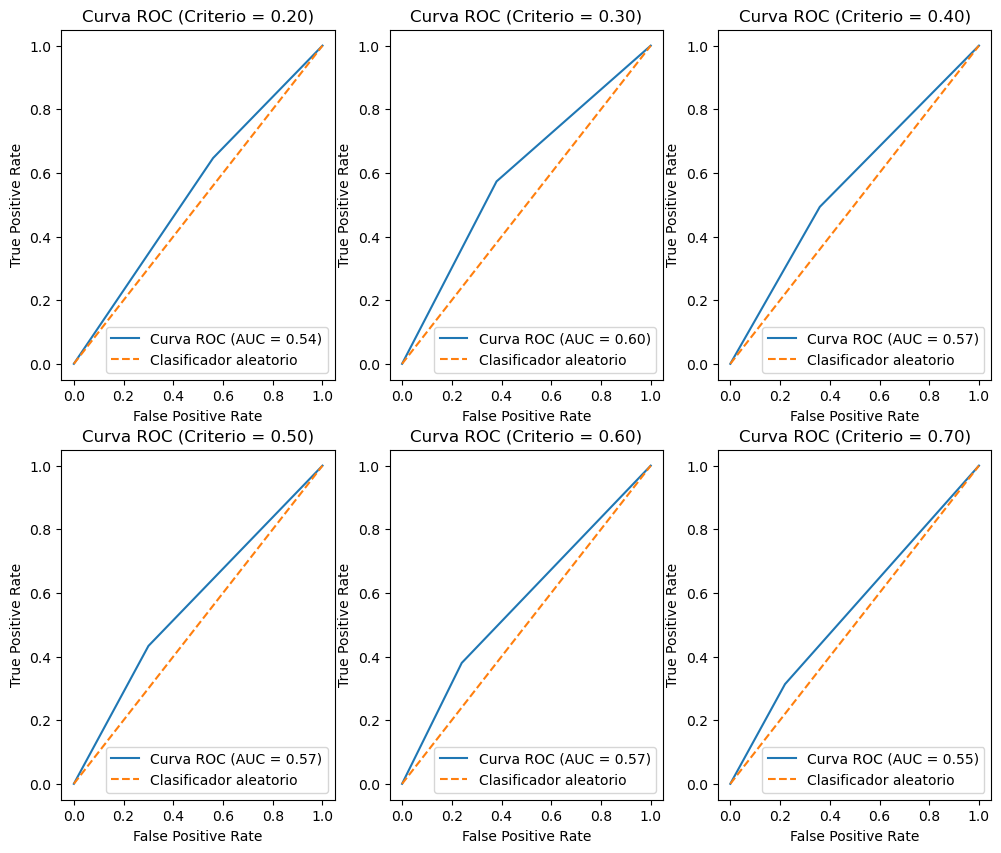
\includegraphics[width=1\textwidth]{img/curvasROC.PNG}
 \caption{Obtención del Mejor Criterio de Clasificación}
 \label{f:curvasROC}
\end{figure}

En tercer lugar, se ha separado una pequeña muestra de los datos originales: 150 registros de la clase NOK y 50 registros de la clase OK. De esta forma, se consigue que ningún modelo haya trabajado antes con estos datos y se puedan evaluar los modelos de una manera más aproximada

En este momento ya se contaba con todo listo para poder realizar diferentes experimentos para construir diferentes conjuntos de modelos, cambiando los parámetros que permiten construir las diferentes redes neuronales para obtener los mejores. Para todos los experimentos se ha seguido la siguiente estrategia:

\begin{itemize}
    \item \textbf{Capa convolucional:} esta capa o capas, según las que se le indiquen, junto con el \emph{kernel} indicado y su activación tipo \emph{relu}, aplican la técnica de convolución a los datos de entrada.
    \item \textbf{Pooling:} aplica la técnica \emph{pooling} y devuelve el valor máximo.
    \item \textbf{Flatten:} transforma los datos de entrada en un vector unidimensional.
    \item \textbf{Dense:} capa o capas que contienen el número de neuronas indicado junto con una activación tipo \emph{relu}.
\end{itemize}

Además, a la hora de entrenar el modelo, se ha utilizado un \emph{checkpoint} para quedarse con el modelo que menor \emph{loss} tenga. También, se pueden modificar el número de iteraciones durante el entreno.

Todo esto aplicando la técnica de validación cruzada y construyendo 5 modelos en cada experimento. Por lo que a la hora de obtener predicciones se sumará la predicción de los 5 modelos y se dividirá entre 5, y finalmente este valor se comparará con el criterio de clasificación, 0.3, y se determinará la clase de la bobina en concreto.

A continuación se recogen los resultados obtenidos tanto para los datos 1D como 2D, y para cada uno de ellos, los resultados obtenidos según si se utiliza solo el mapa codificado de la bobina, o el mapa junto con los demás atributos normalizados.

\subsubsection{Datos 1D}
Se han realizado un total de 7 experimentos para los datos 1D sobre el mapa codificado de la bobina. Los resultados han sido los siguientes:

\begin{itemize}
    \item \textbf{Experimento 1:} en este caso los parámetros utilizados han sido una capa convolucional con 32 filtros , el tamaño de \emph{kernel} es 3, 300 iteraciones, y tres capas densas de tamaños, respectivamente, 32, 8 y 1. Los resultados obtenidos son los siguientes:
    \begin{verbatim}
        La precisión obtenida ha sido 0.535
        La matriz de confusion obtenida es:
         [[27 23]
         [70 80]]
    \end{verbatim}
    \item \textbf{Experimento 2:} en este segundo experimento se han empleado una capa convolucional con 64 filtros y con un \emph{kernel} de tamaño 5. Las iteraciones han sido 500, y las capas densas se han mantenido iguales que en el caso anterior. Los resultados son los siguientes:
    \begin{verbatim}
        La precisión obtenida ha sido 0.54
        La matriz de confusion obtenida es:
         [[30 20]
         [72 78]]
    \end{verbatim}
    \item \textbf{Experimento 3:} en este tercer caso se ha usado una capa convolucional con 16 filtros y con un \emph{kernel} de tamaño 3. Las iteraciones han sido 300, y se han usado 5 capas densas de tamaños 64, 32, 16, 8 y 1. El resultado obtenido ha sido:
    \begin{verbatim}
        La precisión obtenida ha sido 0.54
        La matriz de confusion obtenida es:
         [[29 21]
         [71 79]]
    \end{verbatim}
    \item \textbf{Experimento 4:} en este cuarto caso se ha usado una capa convolucional de 16 filtros y con un \emph{kernel} de tamaño 5. Las iteraciones han sido 300 y se han empleado 3 capas densas de tamaño 32, 8 y 1.  Los resultados obtenidos han sido los siguientes:
    \begin{verbatim}
        La precisión obtenida ha sido 0.56
        La matriz de confusion obtenida es:
         [[29 21]
         [67 83]]
    \end{verbatim}
    \item \textbf{Experimento 5:} en este quinto experimento se han usado 3 capas convolucionales con  16, 32 y 64 filtros y todas ellas con un \emph{kernel} de tamaño 3. Las iteraciones y las capas densas han sido las mimas que las del experimento anterior. Los resultados obtenidos han sido;
    \begin{verbatim}
        La precisión obtenida ha sido 0.57
        La matriz de confusion obtenida es:
         [[32 18]
         [68 82]]
    \end{verbatim}
    \item \textbf{Experimento 6:} en este penúltimo experimento se han mantenido los valores del experimento anterior pero aumentando las iteraciones a 500. Los resultados han sido:
    \begin{verbatim}
        La precisión obtenida ha sido 0.56
        La matriz de confusion obtenida es:
         [[30 20]
         [68 82]]
    \end{verbatim}
    \item \textbf{Experimento 7:} en el último caso se han utilizado los mismos valores que en el experimento 5 pero cambiando el tamaño del \emph{kernel} a 5. Los resultados han sido:
    \begin{verbatim}
        La precisión obtenida ha sido 0.505
        La matriz de confusion obtenida es:
         [[26 24]
         [75 75]]
    \end{verbatim}
\end{itemize}

Sobre el mapa codificado y los atributos normalizados se han realizado otros 7 experimentos, cuyos resultados son los siguientes (en los resultados se incluye la precisión utilizando únicamente el modelo y la precisión obtenida combinando los modelos con el \emph{Random Forest}):

\begin{itemize}
    \item \textbf{Experimento 1:} este primer experimento ha sido con una capa convolucional con 32 filtros y con un \emph{kernel} de tamaño 3. Además, ternía 300 iteraciones y 3 capas densas de tamaños 32, 8 y 1. Los resultados han sido:
    \begin{verbatim}
        La precisión obtenida ha sido 0.47
        La matriz de confusion obtenida es:
         [[35 15]
         [91 59]]
        
        La precisión obtenida con el RF ha sido 0.475
        La matriz de confusion obtenida es:
         [[38 12]
         [93 57]]
    \end{verbatim}
    \item \textbf{Experimento 2:} este segundo caso ha sido igual que el anterior pero con un \emph{kernel} de tamaño 5 y con 16 filtros. Los resultados se muestran a continuación:
    \begin{verbatim}
        La precisión obtenida ha sido 0.51
        La matriz de confusion obtenida es:
         [[33 17]
         [81 69]]
        
        La precisión obtenida con el RF ha sido 0.445
        La matriz de confusion obtenida es:
         [[38 12]
         [99 51]]
    \end{verbatim}
    \item \textbf{Experimento 3:} en este tercer experimento ha sido similar al anterior pero con 64 filtros. Los resultados han sido:
    \begin{verbatim}
        La precisión obtenida ha sido 0.485
        La matriz de confusion obtenida es:
         [[39 11]
         [92 58]]
        
        La precisión obtenida con el RF ha sido 0.46
        La matriz de confusion obtenida es:
         [[40 10]
         [98 52]]
    \end{verbatim}
    \item \textbf{Experimento 4:} este cuarto caso ha sido igual que el primero pero con 16 filtros. Los resultados son:
    \begin{verbatim}
        La precisión obtenida ha sido 0.525
        La matriz de confusion obtenida es:
         [[35 15]
         [80 70]]
        
        La precisión obtenida con el RF ha sido 0.47
        La matriz de confusion obtenida es:
         [[35 15]
         [91 59]]
    \end{verbatim}
    \item \textbf{Experimento 5:} este quinto experimento ha sido igual que el anterior, solo que con 5 capas densas y de tamaños 64, 32, 16, 8 y 1. Se han obtenido los siguientes resultados:
    \begin{verbatim}
        La precisión obtenida ha sido 0.475
        La matriz de confusion obtenida es:
         [[34 16]
         [89 61]]
        
        La precisión obtenida con el RF ha sido 0.455
        La matriz de confusion obtenida es:
         [[40 10]
         [99 51]]
    \end{verbatim}
    \item \textbf{Experimento 6:} este penúltimo experimento ha sido igual que el anterior, pero con dos capas convolucionales con 32 y 64 filtros. Los resultados son:
    \begin{verbatim}
        La precisión obtenida ha sido 0.48
        La matriz de confusion obtenida es:
         [[31 19]
         [85 65]]
        
        La precisión obtenida con el RF ha sido 0.455
        La matriz de confusion obtenida es:
         [[31 19]
         [90 60]]
    \end{verbatim}
    \item \textbf{Experimento 7:} en el último caso, muy parecido al anterior, solo que con un \emph{kernel} de tamaño 5, se han obtenido los siguientes resultados:
    \begin{verbatim}
        La precisión obtenida ha sido 0.425
        La matriz de confusion obtenida es:
         [[ 39  11]
         [104  46]]
        
        La precisión obtenida con el RF ha sido 0.435
        La matriz de confusion obtenida es:
         [[ 43   7]
         [106  44]]
    \end{verbatim}
\end{itemize}

\subsubsection{Datos 2D}
Con respecto a los datos 2D, también se han realizado 7 experimentos sobre los mapas codificados de las bobinas. A continuación se muestran los resultados:

\begin{itemize}
    \item \textbf{Experimento 1:} en este primer caso se utiliza una capa convolucional con 32 filtros y un \emph{kernel} de tamaño 3x3. Además, se efectúan 100 iteraciones y tres capas densas de tamaños 32, 8 y 1. Los resultados han sido los siguientes:
    \begin{verbatim}
        La precisión obtenida ha sido 0.485
        La matriz de confusion obtenida es:
         [[37 13]
         [90 60]]
    \end{verbatim}
    \item \textbf{Experimento 2:} este experimento es muy similar al anterior, solo que con 16 filtros. Los resultados son los siguientes:
    \begin{verbatim}
        La precisión obtenida ha sido 0.49
        La matriz de confusion obtenida es:
         [[37 13]
         [89 61]]
    \end{verbatim}
    \item \textbf{Experimento 3:} este tercer caso es muy similar al primero, pero ahora el tamaño del \emph{kernel} es de 5x5. Sus resultados han sido:
    \begin{verbatim}
        La precisión obtenida ha sido 0.525
        La matriz de confusion obtenida es:
         [[34 16]
         [79 71]]
    \end{verbatim}
    \item \textbf{Experimento 4:} este tercer experimento es similar al primero, pero con 64 filtros. Además, tiene 5 capas densas de tamaños 64, 32, 16, 8 y 1. Sus resultados han sido:
    \begin{verbatim}
        La precisión obtenida ha sido 0.53
        La matriz de confusion obtenida es:
         [[41  9]
         [85 65]]
    \end{verbatim}
    \item \textbf{Experimento 5:} este experimento ha sido similar al primero, solo que con 16 filtros y un \emph{kernel} de tamaño 5x5. Los resultados han sido:
    \begin{verbatim}
        La precisión obtenida ha sido 0.495
        La matriz de confusion obtenida es:
         [[38 12]
         [89 61]]
    \end{verbatim}
    \item \textbf{Experimento 6:} este caso ha sido similar al primero pero con dos capas convolucionales con 16 y 32 filtros. Sus resultados han sido:
    \begin{verbatim}
        La precisión obtenida ha sido 0.49
        La matriz de confusion obtenida es:
         [[36 14]
         [88 62]]
    \end{verbatim}
    \item \textbf{Experimento 7:} este experimento ha sido similar al anterior, pero en este caso con tres capas convolucionales, de tamaños 16, 32 y 64. Los resultados han sido:
    \begin{verbatim}
        La precisión obtenida ha sido 0.54
        La matriz de confusion obtenida es:
         [[34 16]
         [76 74]]
    \end{verbatim}
\end{itemize}

Para los datos 2D juntando el mapa con los demás atributos, se han realizado de igual manera 7 experimentos. Además, al igual que para los datos 1D, se han añadido los resultados de usar \emph{Random Forest}. Todos los resultados se pueden ver a continuación:
\begin{itemize}
    \item \textbf{Experimento 1:} en este primer experimento se utiliza una capa convolucional con 32 filtros y un \emph{kernel} de 3x3. Además, se han empleado 100 iteraciones y 3 capas densas de tamaño 32, 8 y 1. Sus resultados han sido: 
    \begin{verbatim}
        La precisión obtenida ha sido 0.51
        La matriz de confusion obtenida es:
         [[41  9]
         [89 61]]
        
        La precisión obtenida con el RF ha sido 0.5
        La matriz de confusion obtenida es:
         [[42  8]
         [92 58]]
    \end{verbatim}
    \item \textbf{Experimento 2:} este segundo experimento ha sido similar al anterior, pero con 16 filtros y el \emph{kernel} de tamaño 5x5. Los resultados han sido:
    \begin{verbatim}
        La precisión obtenida ha sido 0.505
        La matriz de confusion obtenida es:
         [[30 20]
         [79 71]]
        
        La precisión obtenida con el RF ha sido 0.53
        La matriz de confusion obtenida es:
         [[39 11]
         [83 67]]
    \end{verbatim}
    \item \textbf{Experimento 3:} este caso ha sido muy similar al primero pero con un \emph{kernel} de 5x5. Los resultados han sido:
    \begin{verbatim}
        La precisión obtenida ha sido 0.525
        La matriz de confusion obtenida es:
         [[34 16]
         [79 71]]
        
        La precisión obtenida con el RF ha sido 0.51
        La matriz de confusion obtenida es:
         [[42  8]
         [90 60]]
    \end{verbatim}
    \item \textbf{Experimento 4:} este experimento ha sido como el primero, pero esta vez utilizando 16 filtros. Sus resultados han sido:
    \begin{verbatim}
        La precisión obtenida ha sido 0.49
        La matriz de confusion obtenida es:
         [[40 10]
         [92 58]]
        
        La precisión obtenida con el RF ha sido 0.47
        La matriz de confusion obtenida es:
         [[43  7]
         [99 51]]
    \end{verbatim}
    \item \textbf{Experimento 5:} este experimento ha sido similar al primero, pero las capas densas pasan a ser 5 y sus tamaños son 64, 32, 16, 8 y 1. Sus resultados son:
    \begin{verbatim}
        La precisión obtenida ha sido 0.515
        La matriz de confusion obtenida es:
         [[38 12]
         [85 65]]
        
        La precisión obtenida con el RF ha sido 0.495
        La matriz de confusion obtenida es:
         [[37 13]
         [88 62]]
    \end{verbatim}
    \item \textbf{Experimento 6:} en este sexto caso, similar al primero, se han añadido dos capas convolucionaales con 32 y 16 filtros. Los resultados son:
    \begin{verbatim}
        La precisión obtenida ha sido 0.51
        La matriz de confusion obtenida es:
         [[35 15]
         [83 67]]
        
        La precisión obtenida con el RF ha sido 0.515
        La matriz de confusion obtenida es:
         [[42  8]
         [89 61]]
    \end{verbatim}
    \item \textbf{Experimento 7:} este experimento ha sido similar al anterior, pero con una capa convolucional más. Sus tamaños son 16, 32 y 64, y cuyos resultados son:
    \begin{verbatim}
        La precisión obtenida ha sido 0.49
        La matriz de confusion obtenida es:
         [[39 11]
         [91 59]]
        
        La precisión obtenida con el RF ha sido 0.475
        La matriz de confusion obtenida es:
         [[42  8]
         [97 53]]
    \end{verbatim}
\end{itemize}

\subsubsection{Análisis de resultados}
Para concluir con esta fase, es turno de analizar los resultados que se han obtenido, y que han sido mostrados en los dos subpuntos anteriores.

Lo primero que resalta son los malos resultados, ya que ninguno de los 28 experimentos han mostrado una precisión adecuada, de hecho, casi todos están con una precisión de entre el 50 y 60 porciento, unos resultados para nada aceptables.

Si comparamos los resultados entre los datos 1D y 2D, se ve como las precisiones más altas son las del primer tipo de datos, algo que puede chocar, ya que se puede presuponer que los datos 2D mostrarán algún patrón o característica que haga que el modelo sea mejor, pero no ha sido el caso. Es por ello, que se cree que esto se debe a que en los datos prestados el operario usa para clasificar las bobinas los datos 1D, de ahí esos posibles mejores resultados.

Si comparamos los resultados obtenidos directamente con los modelos a los obtenidos por el \emph{random forest}, se ve como este último, casi siempre es similar o un poco peor que si utilizamos solo el modelo, por lo que no muestra ningún síntoma de ser beneficioso su uso.

Finalmente, el mejor resultado, se ha obtenido con el experimento 5 de los datos 1D empleando tan solo el mapa codificado de la bobina, por lo que será este el que se empleará en la siguiente fase.

\section{Desarrollo de la Aplicación}
En esta sexta y última fase, ha sido turno de construir la aplicación final del proyecto, sobre la cual se puedan cargar datos de bobinas medidos por sensores y predecir y si serán bobinas válidas o no. 

La construcción de la aplicación se ha basado en dos partes. Por un lado, tenemos un \emph{notebook} donde se podrá elegir la base de datos donde se encuentran los datos y visualizar los resultados. Y, por otro lado, tenemos un archivo de \emph{Python} que contiene las diferentes funciones y que encapsula, de cara al usuario, todo el proceso, con el fin de dejar la aplicación lo vas sencilla y visual posible. 

Con respecto a los modelos usados para las predicciones, se han correspondido a los del experimento 5 sobre los datos 1D, ya que, como ya se ha visto en la fase anterior, han sido los que mejores resultados han dado. 

Además, para añadirle más funcionalidad a la aplicación, cada vez que se realizan predicciones sobre un modelo, se genera un archivo CSV que contiene todas las características obtenidas de la bobina, puesto que puede ser interesante almacenar los valores por si fuesen de utilidad al operario. Y también, se ha creado un histórico donde se almacenan las predicciones de las bobinas para poder consultarlas en el futuro sin la necesidad de tener que volver a cargar los datos.

El resultado se puede ver en la Figura \ref{f:apli1}, donde se aprecia la tabla con las diferentes \emph{features} calculadas y el mapa codificado de la bobina. Además, más abajo se puede ver la predicción obtenida por los modelos según los datos obtenidos por cada par de sensores.

\begin{figure}[h]
 \centering
  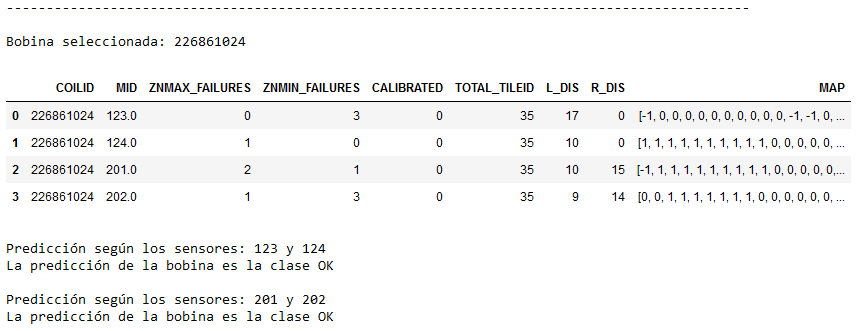
\includegraphics[width=1\textwidth]{img/salidaAp.PNG}
 \caption{Ejemplo de Resultado de la Aplicación}
 \label{f:apli1}
\end{figure}

Y como se ha comentado, se ha generado a su vez un archivo CSV con todos los atributos calculados de la bobina y su mapa codificado para cada sensor. La Figura \ref{f:apli2}, muestra el CSV generado para la bobina de ejemplo mostrada en la imagen anterior. 

\begin{figure}[h]
 \centering
  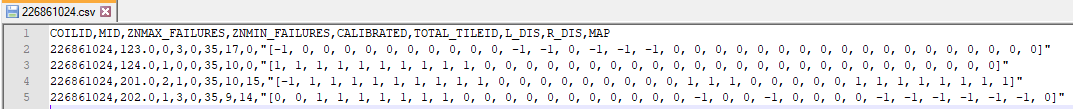
\includegraphics[width=1\textwidth]{img/csv.PNG}
 \caption{Ejemplo de Resultado del CSV Genrado por la Aplicación}
 \label{f:apli2}
\end{figure}

Y también se ha generado un archivo historial.txt que contiene el registro de predicciones. La Figura \ref{f:apli3}, muestra dicho resultado. 

\begin{figure}[h]
 \centering
  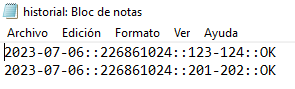
\includegraphics[width=0.5\textwidth]{img/historial.PNG}
 \caption{Ejemplo de Resultado del histroial.txt Genrado por la Aplicación}
 \label{f:apli3}
\end{figure}

Además, si siguiéramos realizando predicciones, se generaría un CSV correspondiente a la bobina y en el fichero correspondiente al historial se añadirían al final la nueva información.